\documentclass[border=6pt]{standalone}
\usepackage{tikz}
\usetikzlibrary{arrows.meta,positioning}
\begin{document}
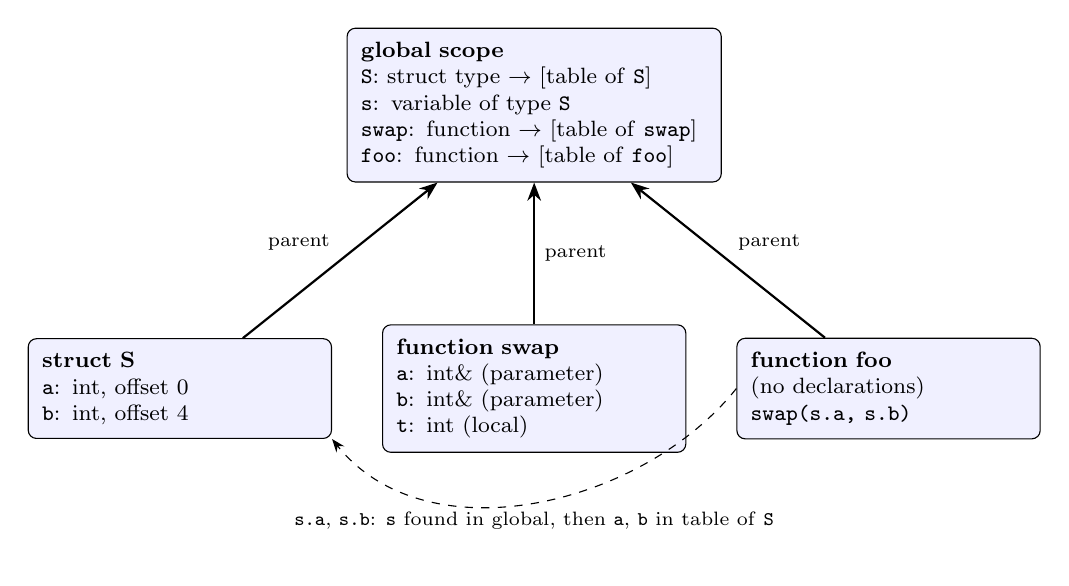
\begin{tikzpicture}[>=Stealth,font=\small,
  tbl/.style={draw,rounded corners=3pt,fill=blue!6,align=left,inner sep=5pt,font=\footnotesize,text width=3.5cm}]
\node[tbl,text width=4.4cm] (G) at (4,0) {\textbf{global scope}\\ \texttt{S}: struct type $\to$ [table of \texttt{S}]\\ \texttt{s}: variable of type \texttt{S}\\ \texttt{swap}: function $\to$ [table of \texttt{swap}]\\ \texttt{foo}: function $\to$ [table of \texttt{foo}]};
\node[tbl] (S) at (-0.5,-3.6) {\textbf{struct S}\\ \texttt{a}: int, offset 0\\ \texttt{b}: int, offset 4};
\node[tbl] (W) at (4,-3.6) {\textbf{function swap}\\ \texttt{a}: int\& (parameter)\\ \texttt{b}: int\& (parameter)\\ \texttt{t}: int (local)};
\node[tbl] (F) at (8.5,-3.6) {\textbf{function foo}\\ (no declarations)\\ \texttt{swap(s.a, s.b)}};
\draw[->,thick] (S) -- node[above left,font=\scriptsize]{parent} (G);
\draw[->,thick] (W) -- node[right,font=\scriptsize]{parent} (G);
\draw[->,thick] (F) -- node[above right,font=\scriptsize]{parent} (G);
\draw[->,dashed] (F.west) .. controls +(-1.2,-1.5) and +(1.2,-1.5) .. node[below,font=\scriptsize]{\texttt{s.a}, \texttt{s.b}: \texttt{s} found in global, then \texttt{a}, \texttt{b} in table of \texttt{S}} (S.south east);
\end{tikzpicture}
\end{document}
